\section{LLMs in Education} 
The growing accessibility of large language models (LLMs) via platforms such as Hugging Face has opened up new possibilities in education for both learners and instructors \cite{wang2024large}. Students increasingly rely on AI to improve learning efficiency, solve problems, and automate routine tasks, while educators explore ways to enhance teaching strategies and content delivery.

Adaptive learning environments aim to tailor educational content and learning strategies to individual learners' needs, preferences, and performance. To dynamically adjust the learning experience, prior research highlights the importance of user modeling, which means tracking learner behavior, progress, and characteristics. Systems typically adapt content difficulty, feedback, and instructional sequencing to improve engagement and learning outcomes. The integration of intelligent agents has proven effective in managing these personalized adjustments \cite{shih2008adaptive}. This foundational work also supports our project's focus on generating synthetic student profiles and aligning content with diverse learner modalities.

\section{Decentralized Training}
Federated learning (FL) \cite{mcmahan2023communicationefficientlearningdeepnetworks} offers a privacy-preserving and communication-efficient solution for training LLMs on decentralized data. Instead of centralizing sensistive datasets, FL enables multiple clients to collaboratively fine-tune a shared model by exchanging only model updates. 

Federated Averaging (FedAvg) \cite{mcmahan2023communicationefficientlearningdeepnetworks}, also refered as Local SGD \cite{stich2019localsgdconvergesfast}, is the standard algorithm in FL. It consists of alternating between a few local
stochastic gradient updates at client nodes, followed by a model averaging update at the server.

Recent frameworks like OpenFedLLM \cite{ye2024openfedllmtraininglargelanguage} have demonstrated the feasability of applying FL to instruction tuning and alignment, two essential components for adapting LLM behavior to user preferences. Using techniques like parameter-efficient fine-tuning (PEFT), these models can be trained effectively across distributed nodes, and even outperforming centralized baselines in domain-specific tasks. In this project, we adopt this paradigm to align LLMs with learner preferences.

\newpage
\section{Preference Alignment} 

\begin{figure*}[h!]
	\center
	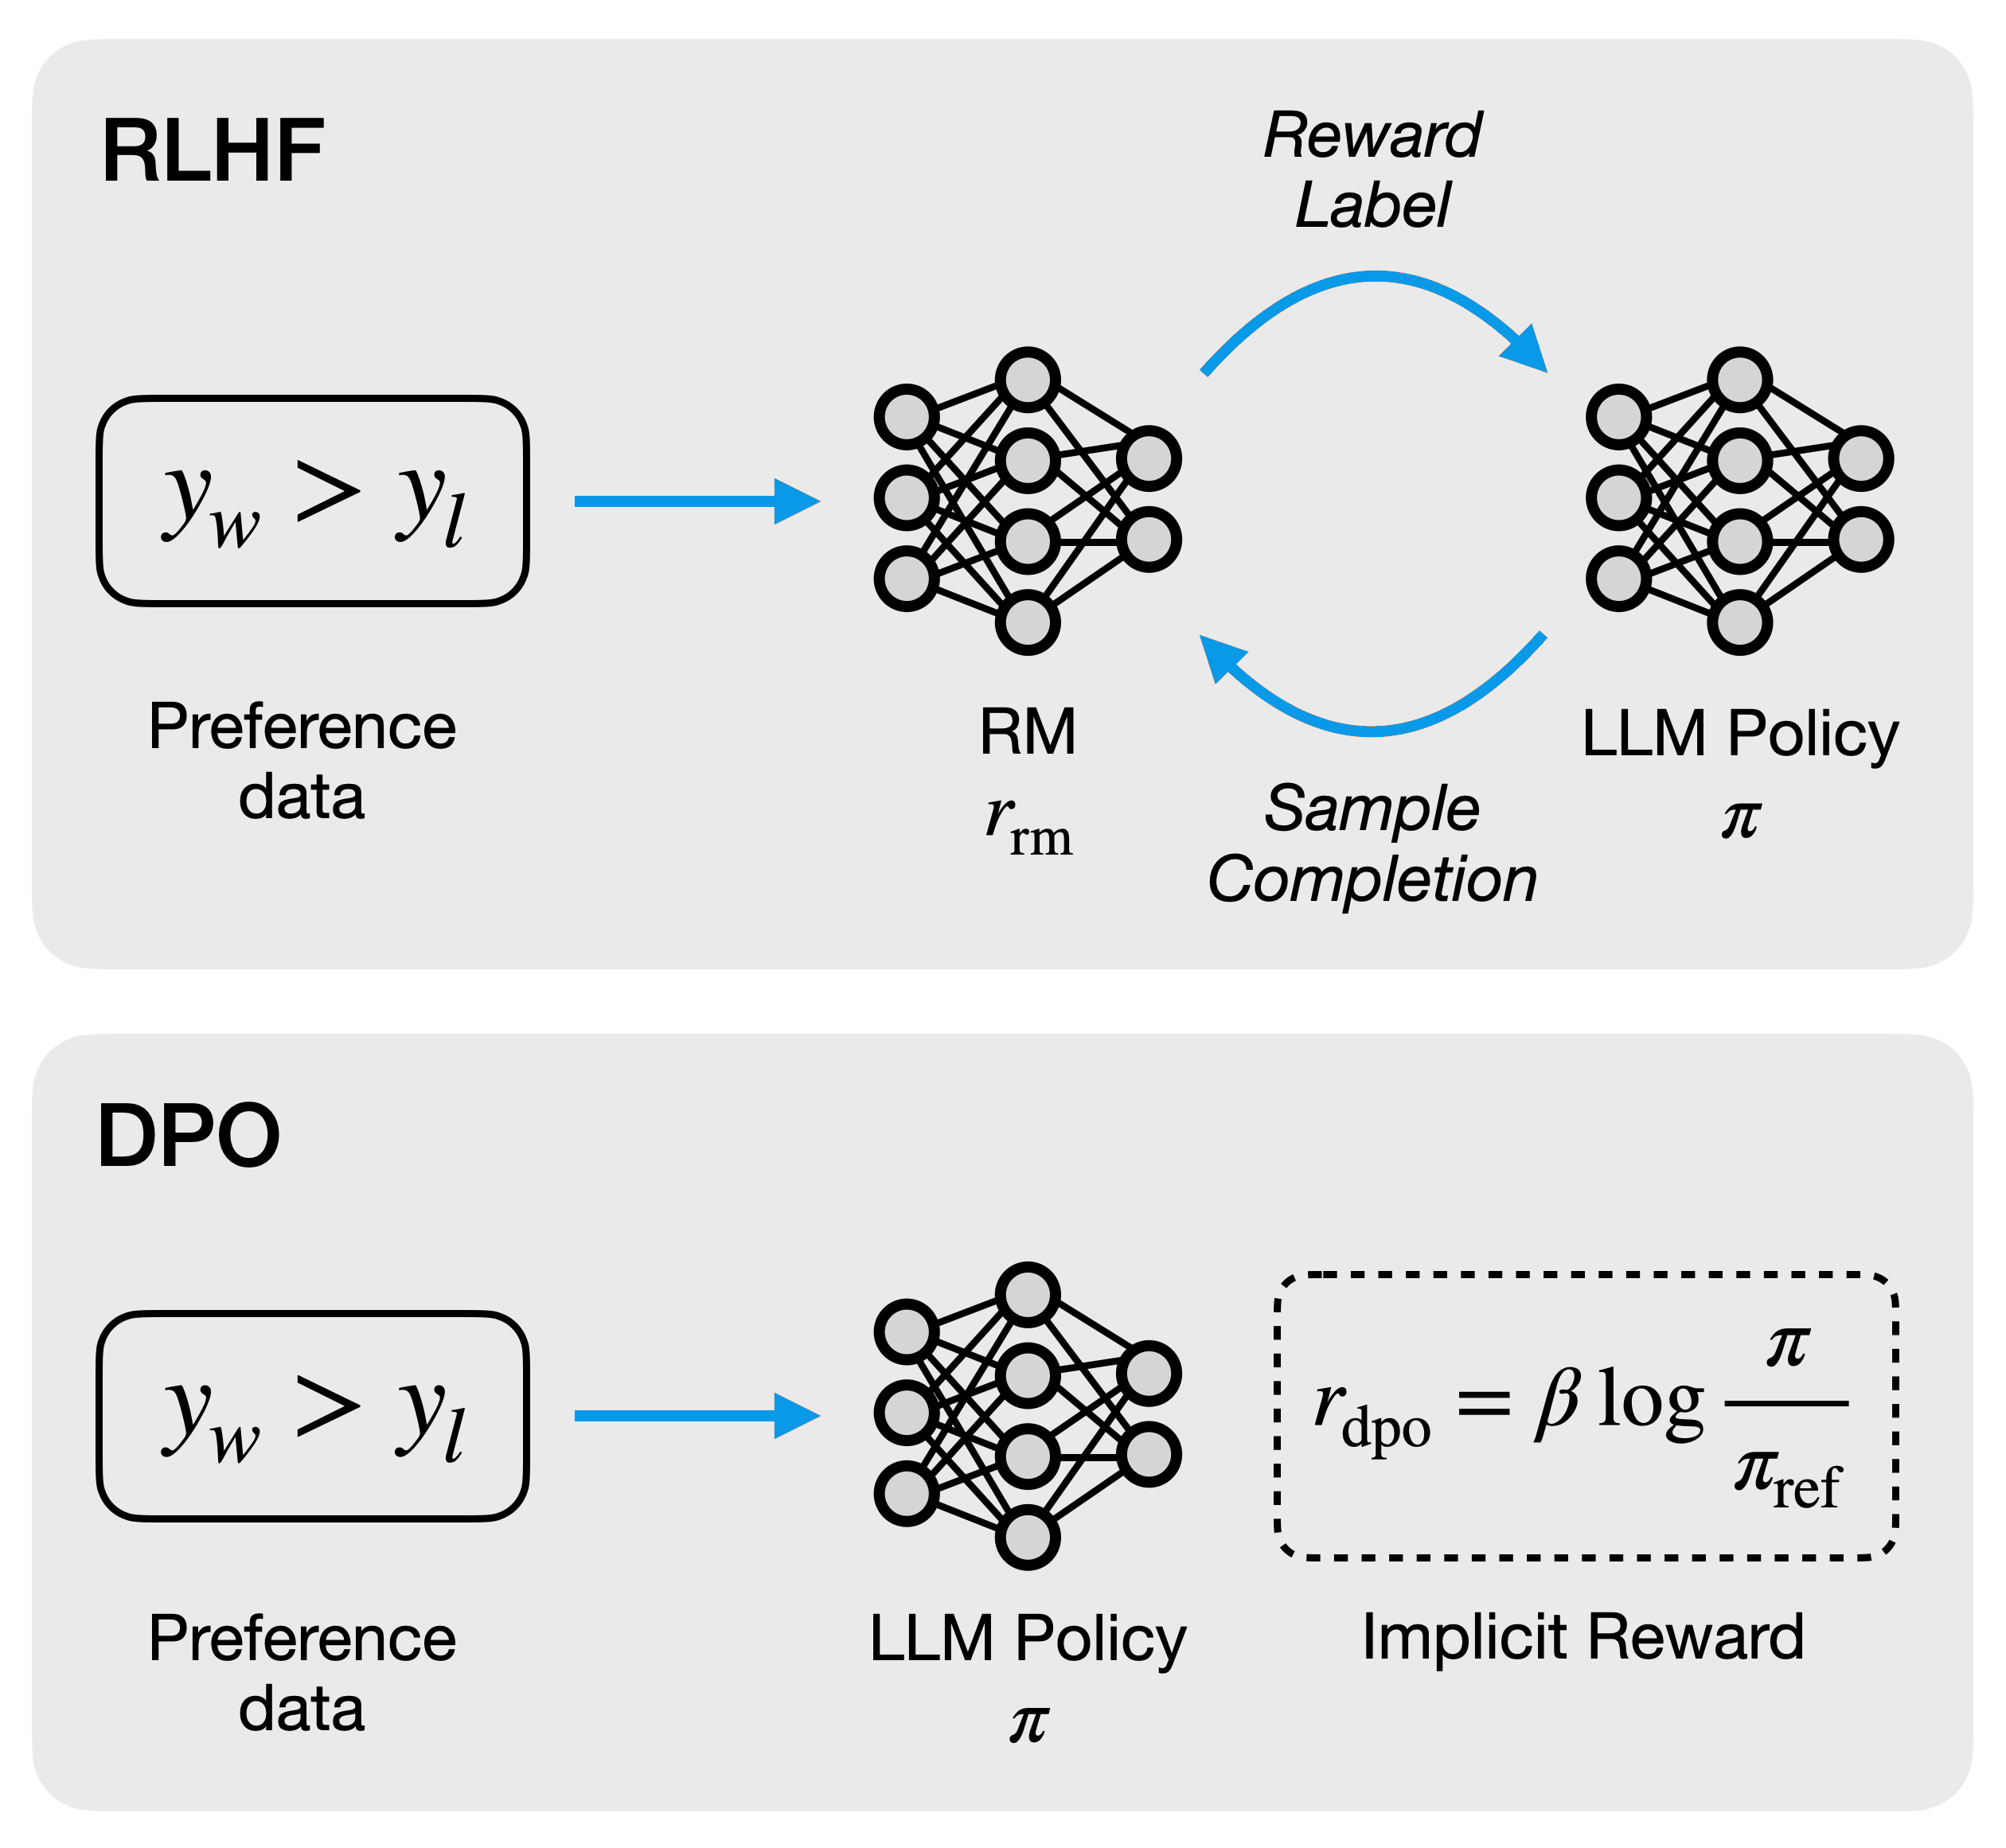
\includegraphics[width=0.6\textwidth]{dpo.png}
	\caption{Comparison between different preference alignment methods. Figure sourced from \cite{lin2024limitedgeneralizationcapabilityimplicit}.}
	\label{fig:dpo}
\end{figure*}

Aligning LLMs with human preferences is key to generating pedagogically effective outputs, especially in educational settings where hallucinations or misinterpretations can harm learning \cite{wang2023aligning}. After supervised fine-tuning (SFT), this alignment is typically achieved through RLHF, a family of methods that optimize models based on preference data.

As illustrated in Figure~\ref{fig:dpo}, two main approaches exist within RLHF. The classic RLHF pipeline involves training a reward model to mimic human preferences, followed by reinforcement learning using algorithms like Proximal Policy Optimization (PPO) \cite{schulman2017proximalpolicyoptimizationalgorithms}. While effective, this setup is complex and prone to instability, as the reward model adds an additional source of bias and potential error in the learning process.

In contrast, Direct Preference Optimization (DPO) \cite{Rafailov2023DirectPO} simplifies the process by eliminating the reward model. Thanks to a supervised contrastive objective, it directly fine-tunes the base model on preference pairs, optimizing a loss that favors preferred responses. The DPO loss has been shown to correspond to a lower bound of the expected KL-regularized reinforcement learning objective that PPO aims to optimize \cite{ivison2024unpackingdpoppodisentangling}. This makes DPO more stable and computationally efficient, while still achieving strong alignment performance \cite{casper2023open}. However, the binary nature of DPO limits its expressivity, making it less capable than PPO of modeling nuanced or continuous preference signals.

For our project, DPO is a better fit, as it only requires constructing a dataset of learning plan preference pairs (each consisting of a chosen and a rejected curriculum) rather than assigning numerical scores to individual plans, which is more subjective and less straightforward. Its simplicity makes DPO well-suited as a robust baseline for preference optimization.

\section{Synthetic data generation} 
Recent advances in machine learning for synthetic data generation have enabled the creation of realistic, high-utility datasets across domains such as healthcare, finance, and education \cite{lu2025machinelearningsyntheticdata}. In education, where access to real user data is often restricted by privacy and ethical concerns, synthetic data provides a practical alternative. It enables experimentation, model training, and benchmarking without the need for large-scale human data. 

Techniques range from classical probabilistic models to deep generative approaches like Generative Adversarial Networks (GANs), diffusion models, and transformer-based architectures (e.g., GPT), often guided by task-specific constraints or utility objectives. In our context, these methods are especially relevant as we aim to simulate both explicit user preferences and implicit behavioral signals. In particular, we use prompting techniques \cite{sahoo2025systematicsurveypromptengineering} to explicitly formulate our data requirements, enabling LLMs to generate structured outputs that adhere to both format and semantic constraints. This approach ensures the generated data is directly usable for downstream RLHF training in our personalized learning pipeline.